\documentclass[iop,numberedappendix,apj,]{emulateapj}

\usepackage{epsfig}
%\usepackage{amsmath}
\usepackage{amsmath,amsthm,amssymb,cases}
\usepackage{rotating}
\usepackage{natbib}
\usepackage{enumerate}
\usepackage{multirow}
\usepackage{array}
\usepackage{appendix}
\usepackage{comment}
\usepackage{color,xcolor}
\usepackage{url}
\usepackage{here}
\usepackage{hyperref}
\hypersetup{colorlinks,linkcolor={blue!50!black},citecolor={blue!50!black},urlcolor={blue!50!black}}
\allowdisplaybreaks[1]
\bibliographystyle{apj}
\renewcommand{\bibname}{References}

\def\plotonesc#1{\centering \leavevmode
\includegraphics[clip=, width=1.70\columnwidth]{#1}}
\def\plotoneh#1{\centering \leavevmode
\includegraphics[clip=, width=.95\columnwidth]{#1}}
\def\plotone#1{\centering \leavevmode
\includegraphics[clip=, width=.85\columnwidth]{#1}}
\def\plotoneShrinkSmall#1{\centering \leavevmode
\includegraphics[clip=, width=.49\columnwidth]{#1}}
\def\plotoneShrinkMed#1{\centering \leavevmode
\includegraphics[clip=, width=.55\columnwidth]{#1}}
\def\plotoneShrinkBig#1{\centering \leavevmode
\includegraphics[clip=, width=.65\columnwidth]{#1}}
\def\plottwo#1#2{\centering \leavevmode
\includegraphics[width=.45\columnwidth]{#1} \hfil
\includegraphics[width=.45\columnwidth]{#2}}
\def\plottwob#1#2{\centering \leavevmode
\includegraphics[width=.49\columnwidth]{#1} \hfil
\includegraphics[width=.49\columnwidth]{#2}}
\def\plottwor#1#2{\centering \leavevmode
\includegraphics[width=.55\columnwidth,angle=90]{#1} \hfil
\includegraphics[width=.55\columnwidth,angle=90]{#2}}
\def\plotthree#1#2#3{\centering \leavevmode
\includegraphics[width=.3\columnwidth]{#1} \hfil
\includegraphics[width=.3\columnwidth]{#2} \hfil
\includegraphics[width=.3\columnwidth]{#3}}

\def\gsim{\;\rlap{\lower 2.5pt
 \hbox{$\sim$}}\raise 1.5pt\hbox{$>$}\;}
\def\lsim{\;\rlap{\lower 2.5pt
   \hbox{$\sim$}}\raise 1.5pt\hbox{$<$}\;}
%\def\fast{\;$f^{\ast }$\;}
\def\fast{\tilde f}

% set formatting properties
\setlength{\textwidth}{6.5in}
\setlength{\textheight}{8.8in}
\setlength{\hoffset}{0.0in}
\setlength{\voffset}{-0.4in}
\parindent 0.2in
\parskip 0.1in

\def\memoYF#1{\color{red}[YF: {\bf #1}]\color{black}}
\def\memoJLY#1{\color{green}[JLY: {\bf #1}]\color{black}}
\def\memoNBC#1{\color{blue}[NBC: {\bf #1}]\color{black}}



%%% http://www.oceanwave.jp/index.php?float%B4%C4%B6%AD(figure%2Ftable)%A4%CE%BD%D0%CE%CF%B0%CC%C3%D6%A4%F2%A5%B3%A5%F3%A5%C8%A5%ED%A1%BC%A5%EB

%%%%%%%%%%%%%%%%%%%%%%%%%%%%%%%%%%%%%%%%%%%%%%%%%
% THE DOCUMENT BEGINS HERE                      %
%%%%%%%%%%%%%%%%%%%%%%%%%%%%%%%%%%%%%%%%%%%%%%%%%

%\slugcomment{Submitted to ApJ, XX September 2015}

\begin{document}

\title{Rotational Spectral Unmixing of Exoplanets:\\Degeneracies between Surface Colors and Geography}


\author{
%
Yuka Fujii\altaffilmark{1,2} 
%
Jacob Lustig-Yaeger\altaffilmark{3,4,5} 
%
Nicolas B. Cowan\altaffilmark{6,7} 
%
}

\affil{$^1$NASA Goddard Institute for Space Studies, 
  New York, NY 10025, USA}
      
\affil{$^2$Earth-Life Science Institute, Tokyo Institute of Technology, 
  Tokyo, 152-8550, JAPAN}
  
\affil{$^3$Astronomy Department, University of Washington, Box 951580, Seattle, WA 98195, USA}

\affil{$^4$Astrobiology Program, University of Washington, 3910 15th Ave. NE, Box 351580, Seattle, WA 98195, USA}

\affil{$^5$NASA Astrobiology Institute -- Virtual Planetary Laboratory Lead Team, USA}

\affil{$^6$Department of Earth and Planetary Sciences, McGill University, Montreal, Quebec
Canada H3A 0E8}

\affil{$^7$Department of Physics, McGill University, Montreal, Quebec
Canada H3A 0E8}



\vspace{0.5\baselineskip}

\email{
yuka.fujii.ebihara@gmail.com
}

\begin{abstract}

\end{abstract}

\keywords{planets and satellites: surfaces --- planets and satellites: terrestrial planets}
  
%]%%% End front material



%%%%%%%%%%%%%%%%%%%%%%%%%%%%%%%%%%%%%%%%%%%%%%%%%%%%%%%%%%%%%%%%%%%
\section{Introduction}
\label{sec:intro}
%%%%%%%%%%%%%%%%%%%%%%%%%%%%%%%%%%%%%%%%%%%%%%%%%%%%%%%%%%%%%%%%%%%

Direct imaging is expected to play a vital role in characterizing Earth analogs in habitable zones and beyond. 
Substantial work has gone into prediciting detectable features in disk-integrated spectra of the Earth and other planets, as they are observed from an astronomical distance. 
Atmospheric molecules are identifiable through spectral absorption features \citep[e.g.,][]{DesMarais2002} but surface reflectance spectra also affect the spectra, which could be measured through low-resolution spectra, or multi-band photometry \citep[e.g.,][]{Ford2001}. 
However, interpreting disk-integrated colors is not trivial. 
This is particularly true for Earth-like planets that harbor diverse atmospheric and surface characteristics including liquid water, partial cloud cover, continents, and possibly vegetation. 

A key here is to leverage the time variation of the spectrum: the regions that contributes to the scattered light change due to the planetary rotation and  orbital motion, so the time variability can in principle be translated to the heterogeneity of the surface environment.  
\citet{Cowan2009, Cowan2011} performed Principal Component Analysis (PCA) on the observed multi-band photometry of Earth. They found that the number of surface types can be inferred from the number of dominant principle components: (\# of surface types) $\ge $ (\# of principal components) $+ 1$. %) and that the variation pattern is indicative of the surface properties. 
\citet{Fujii2010, Fujii2011} decomposed multi-band photometric data of the Earth assuming the template reflectance spectra of the known major surface types, and they found that the relative abundance and the longitudinal variation of these surface types are approximately recovered. 
Moreover, by coupling the time variation due to rotation with phase variation due to orbital revolution, a 2-dimensional information of the surface may be retrieved \citep{Kawahara2010, Kawahara2011, Fujii2012}. 

\citet{Cowan2013} took another approach to the same inverse problem. 
Their strategy was to try to estimate the reflectance spectra if surfaces and their distribution across the globe simultaneously, by making all of them fitting parameters. 
The result appeared successful to the extent that the obtained reflectance spectra roughly match the average spectra of clouds, ocean, and continents. 
However, the longitudinal map of these components did not match the actual geographyical distribution of surfaces. 

We were motivated by this unsatisfactory result to revisit their analysis. 
Specifically, the updates are (1) Revisiting the formulation and point out the inherit degeneracy between surface spectra and geography, and (2) Introducing regularization terms to enforce smooth longitudinal maps. 
We limit our discussions to the analysis of noise-free data. Clearly, noise in realistic observations of exoplanets are expected to be substantially larger, and the effect of such observations will be discussed elsewhere. 

The organization of this paper is as follows. 
Section \ref{s:frame} revisits the problem, ....

%\newpage

%%%%%%%%%%%%%%%%%%%%%%%%%%%%%%%%%%%
\begin{figure}[t]
    \begin{center}
	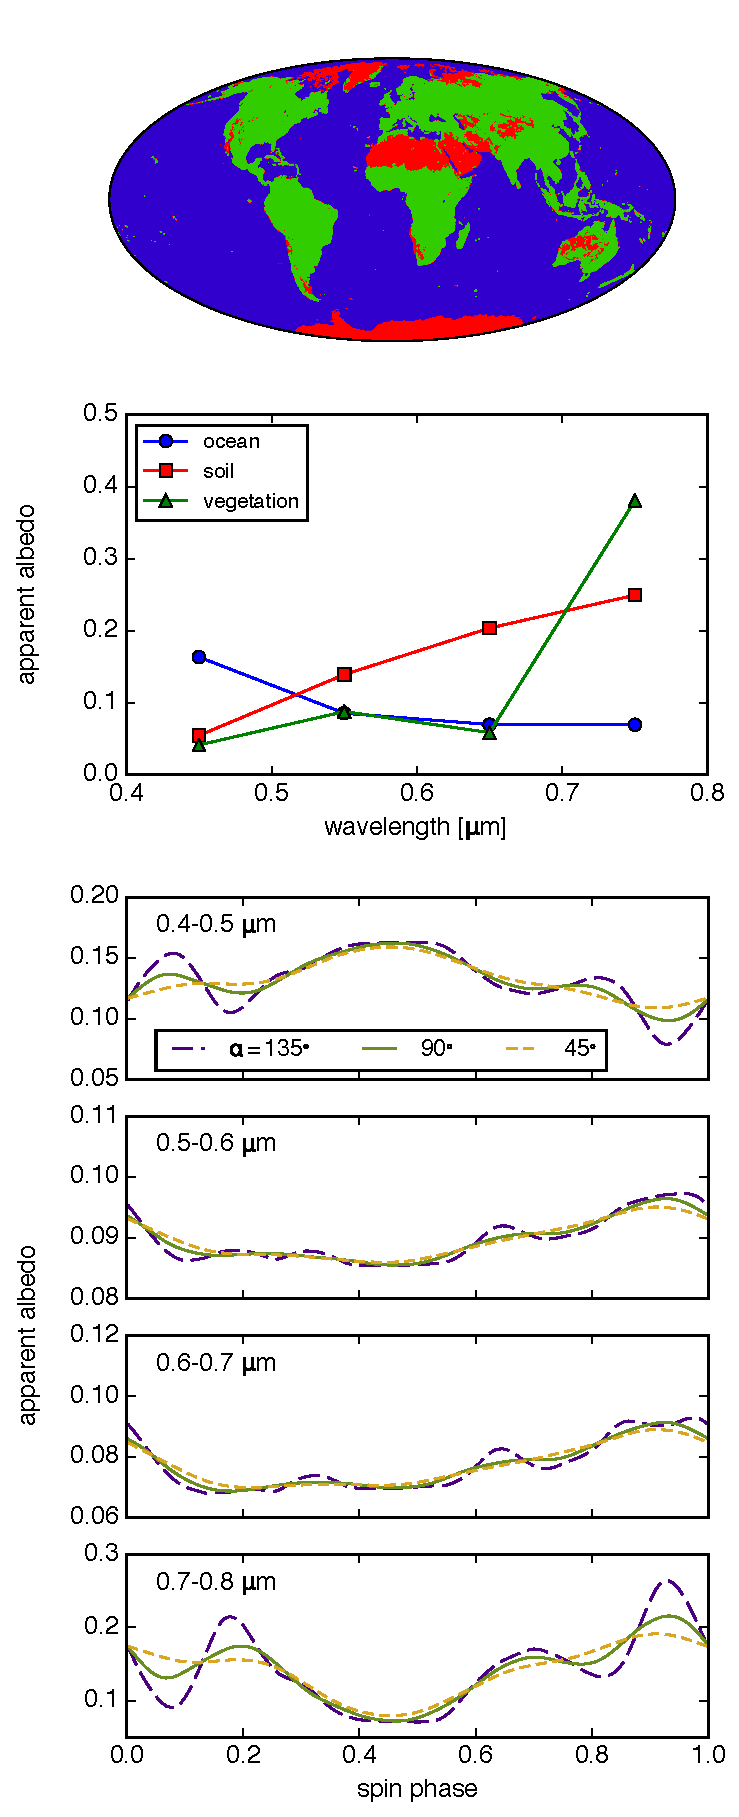
\includegraphics[width=\hsize]{mockdata.pdf}
%    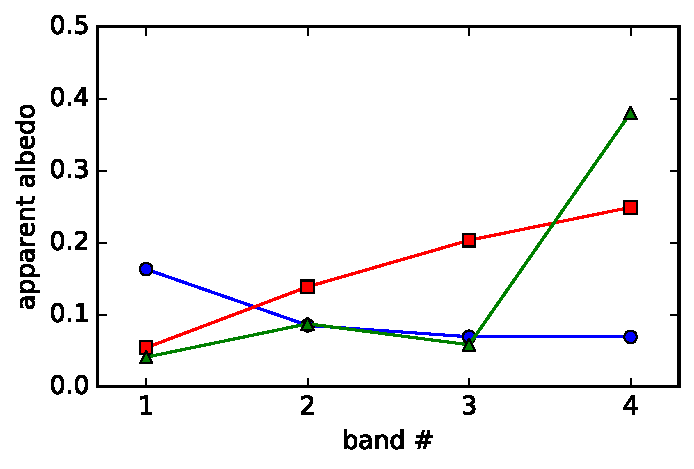
\includegraphics[width=\hsize]{mockdata_3types_albd.pdf}
%	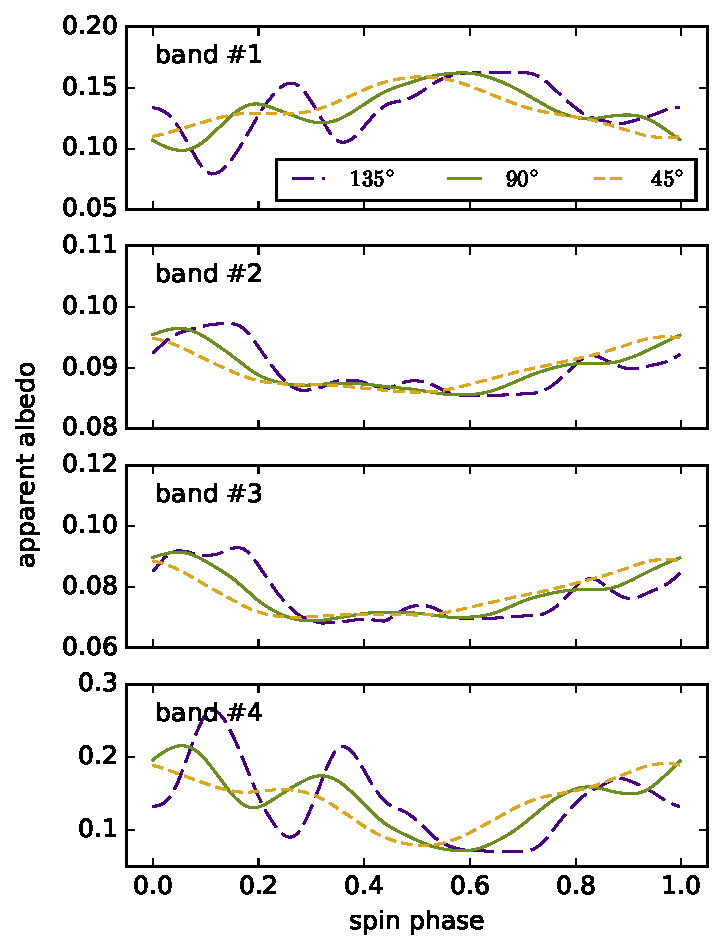
\includegraphics[width=\hsize]{mockdata_3types_t360_lc.pdf}
    \end{center}
    \caption{Our mock data based on IGBP classification map of the Earth. Top panel: distribution of 3 surface types (ocean: blue, soil: red, vegetation: green). Middle panel: assumed albedo spectra with matching colors. Bottom 4 panels: rotational light curves in 4 photometric band with varying phase angle, $\alpha = 135^{\circ }$ (purple, dot-dashed), $90^{\circ }$ (olive, solid), and $45^{\circ }$ (gold, dashed). }
\label{fig:mockdata}
\end{figure}
%%%%%%%%%%%%%%%%%%%%%%%%%%%%%%%%%%%


%%%%%%%%%%%%%%%%%%%%%%%%%%%%%%%%%%%%%%%%%%%%%%%%%%%%%%%%%%%%%%%%%%%
\section{Preparing Mock Datasets}
\label{s:mockdata}
%%%%%%%%%%%%%%%%%%%%%%%%%%%%%%%%%%%%%%%%%%%%%%%%%%%%%%%%%%%%%%%%%%%

%The aim of this paper is to present how to constrain the albedo spectra of representative surface types from multi-band light curves. 
In order to facilitate the discussions in the following sections about the procedures to constrain the albedo spectra of representative surface types from multi-band light curves, we shall introduce a dataset to be used for demonstrations in this section. 

We consider diurnal light curves of a toy model of the atmosphere-less Earth, in 4 photometric bands. 
We use a simplified surface map as shown in the upper left panel of Figure \ref{fig:mockdata}. 
This map is based on the land classification by the International Geosphere-Biosphere Programme (IGBP)\footnote{\url{https://climatedataguide.ucar.edu/climate-data/ceres-igbp-land-classification}}. 
Although the original classification assumes 16 land surface types plus ocean, in this paper we assume 3 surface types for simplicity regarding ``Open Shrubs'', ``Urban'', ``Snow/Ice'', and ``Barren/Desert'' as ``soil'' (red in the upper left panel of Figure \ref{fig:mockdata}) and other land surface types as ``vegetation'' (green), while keeping the ``ocean'' regions. 


The assumed albedo spectra of these surface types in 4 photometric bands are shown in the upper right panel of Figure \ref{fig:mockdata}. 
These 4 photometric bands actually correspond to the 0.4-0.5 $\mu $m, 0.5-0.6 $\mu $m, 0.6-0.7 $\mu $m, and 0.7-0.8 $\mu $m, respectively, but they will be simply called by the band indices unless otherwise noted. \memoJLY{I think it would be helpful to make the "band \#"-axis wavelength in microns, and then perhaps refer to the band \# in the text or in an upper x-axis. }
The albedo spectrum for ocean is based on \citet{Mclinden1997}, 
and the data for soil and vegetation are taken from ASTER spectral library\footnote{\url{https://speclib.jpl.nasa.gov/}. 
Specifically, we adopt  ``Brown to dark brown sand'' for ``soil'', and ``Grass'' for the ``vegetation''}. 
The scattering phase function by the surface is assumed to obey the Lambert law, i.e., the radiance is (incident flux)$\times $(albedo)/$\pi$, independent of the direction of the scattering. 
Note that in reality they are not Lambertian scatterers; among others,  scattering by ocean is very anisotropic.  

% and the albedo spectra of ocean overlaid with atmosphere  
%\memoJLY{A phase of 135 deg is right in the range that Ty (Robinson et al. 2010; 2011) shows will deviate most from a Lambertian scatterer due the ocean glint...}

The light curves are synthesized given the relative potisions of the star, planet, and observer.  
For the sake of simplicity, we consider a planet with zero obliquity in an edge-on orbit, and change the phase angle (the planet-centric angle between the star and the observer) denoted by $\alpha $. 
However, the following discussion does not depend on these assumptions. 

The bottom panels of Figure \ref{fig:mockdata} display the examples of diurnal light curves in 4 photometric bands, represented in terms of {\it apparent albedo}. 
Apparent albedo is the planetary intensity normalized by that of a loss-less Lambert sphere with the same radius and at the same phase \citep{Qiu2003, Seager2010}; in this paper we will use apparent albedo unless otherwise noted. 
The apparent albedo is straightforwardly obtained from the observed planetary intensity, if and only if the planetary radius and the observational geometry are completely known: latitude/longitude of the sub-stellar/sub-observer points, and the distance between the star and the planet. 
%\memoYF{Later in the paper, mention that the uncertainty in radius estimation severely affects the constraints. }
%(We will discuss the effect of this assumptions later in Section ??.)

The problem throughout this paper is, from this kind of multi-band diurnal light curves, how and how well we can retrieve the albedo spectra of different surface types as well as the longitudinal distribution of these surface types. 


%%%%%%%%%%%%%%%%%%%%%%%%%%%%%%%%%%%%%%%%%%%%%%%%%%%%%%%%%%%%%%%%%%%
\section{Inverse problem}
\label{s:frame}
%%%%%%%%%%%%%%%%%%%%%%%%%%%%%%%%%%%%%%%%%%%%%%%%%%%%%%%%%%%%%%%%%%%

In this section, we discuss the general framework to analyze the diurnal light curves, and present some demonstrations using the mock data created in the previous section. 
Sections \ref{ss:model} and \ref{ss:PCplane} are essentially the recapitulation of the previous papers, in particular \citet{Cowan2013} \citep[but see also][]{Cowan2009,Cowan2011,Fujii2010,Fujii2011}.  
We, however, choose to include these discussions as a baseline to establish the later arguments. 
\memoYF{Too many overlaps??}

%%%%%%%%%%%%%%%%%%%%%%%%%%%%%%%%%%%%%%%%%%%%%%%%%%%%%%%%%%%%%%
\subsection{Algebraic Formulation}
\label{ss:model}
%%%%%%%%%%%%%%%%%%%%%%%%%%%%%%%%%%%%%%%%%%%%%%%%%%%%%%%%%%%%%%


%%%%%%%%%%%%%%%%%%%%%%%%%%%%%%%%%%%
\begin{table}[b]
\caption{Indexes}
\begin{center}
\begin{tabular}{lcc} \hline \hline
Name & Symbol & Maximum \\ \hline
Observation Time & $i$ & I \\
Band & $j$ & J  \\
Surface Type & $k$ & K  \\
Longitudinal Slice  & $l$ & L \\ \hline
\end{tabular}
\end{center}
\label{tab:index}
\end{table}%
%%%%%%%%%%%%%%%%%%%%%%%%%%%%%%%%%%%


On the assumption that the planetary surface is Lambertian scatterer everywhere, and that it is composed of a certain number $K$ of spectrally distinct surface types, the disk-integrated scattered light is a weighted summation of the reflectance spectra of different surface types. 
Using the local surface albedo $s_{\vec \Omega }$, the zenith angle of the insolation, $\theta _0$, and the zenith angle of the observer $\theta _1$ (both defined at each surface point),
the apparent albedo of the planet, $d_{ij}$ (``$d$'' for data) is written as follows \citep[see][]{Fujii2010}: 
%%%
\begin{eqnarray}
d_{i} (\lambda_j) &=& \displaystyle \frac{ \int_{{\rm IV}_i} s_{\vec \Omega }(\lambda_j) \cdot \cos \theta_0 ({\vec \Omega}) \cdot \cos \theta_1 ({\vec \Omega}) \cdot d\vec \Omega }{ \int_{{\rm IV}_i}  \cos \theta_0 ({\vec \Omega}) \cdot \cos \theta_1 ({\vec \Omega}) \cdot d\vec \Omega } \\
&=& \sum _{k} s_k (\lambda_j) \; \displaystyle \frac{ \int_{{\rm IV}_{i}} f_k (\vec \Omega ) \cos \theta_0 ({\vec \Omega}) \cdot \cos \theta_1 ({\vec \Omega}) \cdot d\vec \Omega }{ \int_{{\rm IV}_i}  \cos \theta_0 ({\vec \Omega}) \cdot \cos \theta_1 ({\vec \Omega}) \cdot d\vec \Omega } \notag \\
&=& \sum _{i,k} \fast_{ik} \, s_{kj} \label{eq:tilde_d_f_ast_s}
\end{eqnarray}
%%%
where the surface spectra are:
%%%
\begin{equation}
s _{kj} \equiv  s_k (\lambda _j)
\end{equation}
%%%
and the apparent cover fractions are:
%%%
\begin{equation}
\tilde f_{ik} \equiv  \frac{ \int_{{\rm IV}_{i}} f_k (\vec \Omega ) \cos \theta_0 ({\vec \Omega}) \cdot \cos \theta_1 ({\vec \Omega}) \cdot d\vec \Omega }{ \int_{{\rm IV}_i}  \cos \theta_0 ({\vec \Omega}) \cdot \cos \theta_1 ({\vec \Omega}) \cdot d\vec \Omega }
\end{equation}
%%%
and $i$, $j$, and $k$ are indices for the observation epochs, bands, and the surface types, respectively, ${\rm IV }_i$ denotes the illuminated and visible area over the planetary surface at $i$-th observation, and $f (\vec \Omega )$ is the area fraction of $k$-th surface type in $d\vec \Omega$. 
In the last expression, $\fast_{ik}$ represents the apparent covering fraction of the $k$-th surface type at $i$-th observational epoch, and 
$s_{kj}$ is the reflectance spectra of $k$-th surface type at $j$-th band. 
The maximum number of $i$, $j$ and $k$ will be denoted by $I$, $J$, and $K$, below, as summarized in Table \ref{tab:index}. 

By definition, the area fraction, $\fast $, should not be negative and sum up to unity, and reflectance spectra, $s$, should be between 0 and 1. Therefore,
%%%
\begin{subnumcases}
{}
0 \leq \fast_{lk} \;\;\; & \mbox{for any $l$, $k$} \label{eq:tilde_f_range} \\
\sum_k \fast_{lk} = 1 & \mbox{for any $l$} \label{eq:tilde_f_sum} \\
0 \leq s_{kj} \leq 1 \;\;\; & \mbox{for any $k$, $j$} \label{eq:tilde_s_range} 
\end{subnumcases}
%%%


%%%
%\begin{eqnarray}
%\begin{cases}
%\;\; 0 \leq s_{kj} \leq 1 \;\;\; & \mbox{for any $k$, $j$} \\
%\;\; 0 \leq \fast_{lk} \leq 1 \;\;\; & \mbox{for any $l$, $k$} \label{eq:cond_f_ast}\\
%\;\; \sum_k \fast_{lk} = 1 & \mbox{for any $l$} 
%\end{cases}
%\end{eqnarray}
%%%

%\subsection{Estimating the Composition\\of Longitudinal Slices}

The time variability of the apparent covering fraction $\fast $ due to the planet's rotation is related to the surface inhomogeneity along the equator. Approximately, $\fast _{ik}$ may be written as the weighted summation of the area fraction of $k$-th surface type in each of (the finite number $L$ of) longitudinal slices, i.e.,
%%%
\begin{eqnarray}
\fast _{ik} &=& \frac{ \int f_k (\vec \Omega ) \cos \theta_0 ({\vec \Omega}) \cdot \cos \theta_1 ({\vec \Omega}) \cdot d\vec \Omega }{ \int_{{\rm IV}_i}  \cos \theta_0 ({\vec \Omega}) \cdot \cos \theta_1 ({\vec \Omega}) \cdot d\vec \Omega }  \\
&=& \sum_l \frac{ \int f_k (\vec \Omega ) W_i (\vec \Omega  ) \cdot d\vec \Omega }{ \int  W_i (\vec \Omega ) \cdot d\vec \Omega } \\
%&\approx & \sum_l f_{lk} \frac{ \int W_i (\vec \Omega ) \cdot d\vec \Omega }{ \int  W_i (\vec \Omega ) \cdot d\vec \Omega } \label{eq:discretize}\\
&\approx & \sum_l  W_{il} f_{lk} \label{eq:Wf}, \\
W_{il} &\equiv & \frac{ \int  W_i (\vec \Omega  ) \cdot d\vec \Omega_l }{ \int W_i (\vec \Omega )  \cdot d\vec \Omega }
\end{eqnarray}
%%%

where $l$ is the index for longitudinal slices, $f_{lk}$ is the area fraction of the $k$-th surface type in the $l$-th longitudinal slice. 
Strictly speaking, the approximation is valid only when $f_k(\vec \Omega)$ does not change or changes little across the $l$-th slice for all $k$ and $l$. 
\memoNBC{Is this approximation exact in the zero obliquity, edge-on limit?} \memoYF{I don't think so. It is due to pixelization, and does not depend on geometry, I think. ( Perhaps am I not understanding your question properly?) If we suppose the equation were exact, 
%%%
\begin{eqnarray}
f_{lk} &=& \frac{ \int f_k (\vec \Omega ) W_i (\vec \Omega  ) \cdot d\vec \Omega_l }{ \int W_i (\vec \Omega )  \cdot d\vec \Omega_l }\\
\end{eqnarray}
%%%
} 
In the last equation, $W_{il}$ is the weight function for $i$-th epoch and $l$-th longitudinal slice which depends only on the observational geometry. 
As a result,
%%%
\begin{equation}
d_{ij} = \sum _{l,k} W_{il} \, f_{lk} \, s_{kj} \label{eq:d_f_s}
\end{equation}
%%%
where $f_{lk}$ is the average area fraction of $k$-th surface type at $l$-th longitudinal slice, Again, the area fractions at longitudinal slices, $f_{lk}$, cannot be negative and should sum up to unity. Thus, a set of condition similar to Equations (\ref{eq:tilde_s_range})-(\ref{eq:tilde_f_sum}) are imposed:
%%%
\begin{subnumcases}
{}
0 \leq f_{lk} \;\;\; & \mbox{for any $l$, $k$} \label{eq:f_range} \\
\sum_k f_{lk} = 1 & \mbox{for any $l$} \label{eq:f_sum} \\
0 \leq s_{kj} \leq 1 \;\;\; & \mbox{for any $k$, $j$} \label{eq:s_range}
\end{subnumcases}
%%%
Now, the relevant problem is, given $d$, estimate $\{f, s\}$ subject to the constraints of Equations (\ref{eq:s_range})-(\ref{eq:f_sum})---this is where \citet{Cowan2013} stood. 


%\citet{Cowan2013} proposed the specific procedure to find the solution for $\{f, s\}$. 
%Namely, 
%(1) perform PCA on the data to reduce the dimensionality as needed, 
%(2) perform simplex shrink-wrapping analysis to find the first guess for $s$, 
%and 
%(3) find the maximum posterior values for $\{f, s\}$ using MCMC algorithm  and setting the first guess for $s$ as the initial condition. 
%(The initial value for $f$ is fixed at 1/(\# of surface types).)

%\newpage


%%%%%%%%%%%%%%%%%%%%%%%%%%%%%%%%%%%
\begin{figure}[b!]
    \begin{center}
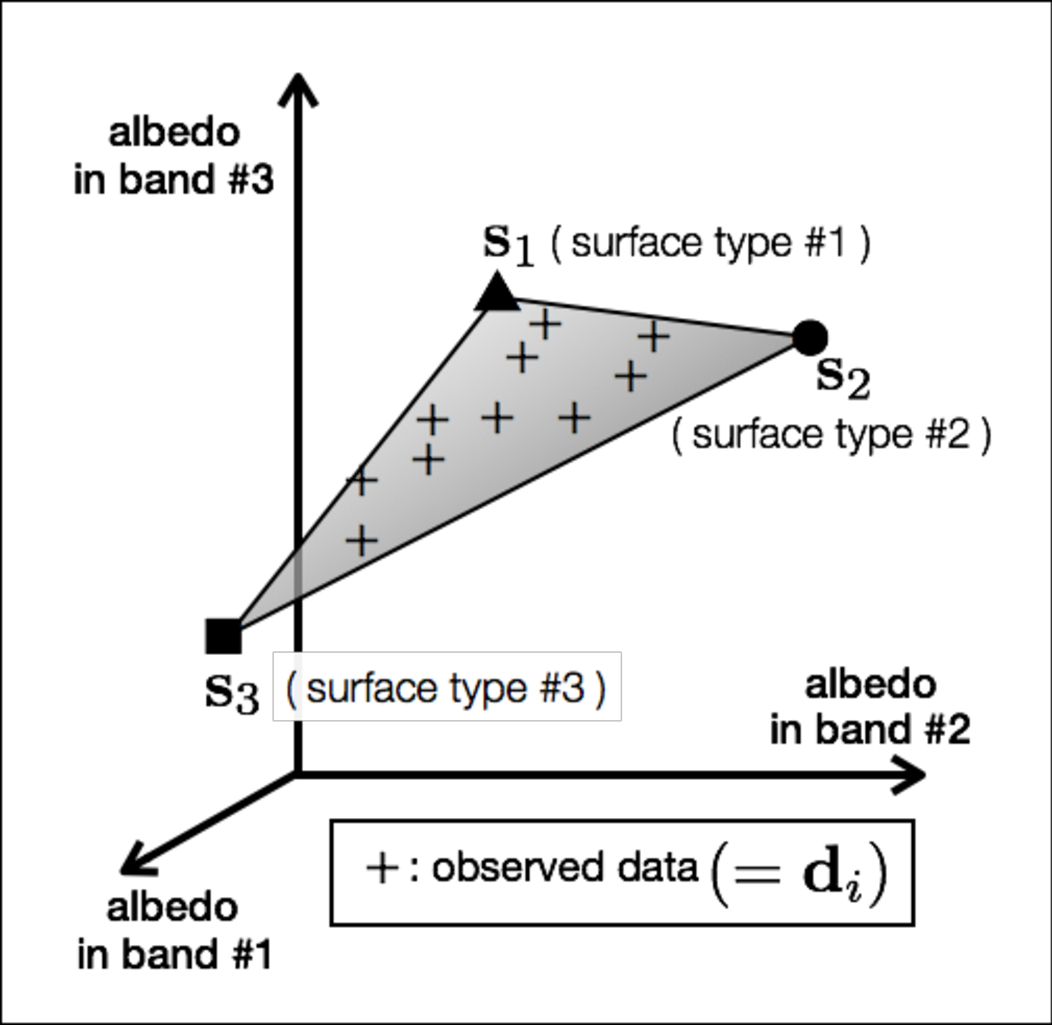
\includegraphics[width=\hsize]{schematics.pdf}
    \end{center}
    \caption{Schematic figure to illustrate the relation between $\{{\bf s}_k\} $ and $\{{\bf d}_i\} $ (see text). }
\label{fig:schematic}
\end{figure}
%%%%%%%%%%%%%%%%%%%%%%%%%%%%%%%%%%%


%%%%%%%%%%%%%%%%%%%%%%%%%%%%%%%%%%%%%%%%%%%%%%%%%%%%%%%%%%%%%%
\subsection{Graphical Conception on \\Principal Component (Hyper-)Plane}
\label{ss:PCplane}
%%%%%%%%%%%%%%%%%%%%%%%%%%%%%%%%%%%%%%%%%%%%%%%%%%%%%%%%%%%%%%

%A question is whether the above formulation leads us to a unique solution of either $\{ {\bf \fast},\,{\bf s} \}$ or $\{ {\bf f},\,{\bf s}\}$, given the data matrix, ${\bf d}$. 

Equation (\ref{eq:tilde_d_f_ast_s}) coupled with the conditions (\ref{eq:tilde_f_range}) and (\ref{eq:tilde_f_sum}) indicates the geometrical relationship among ${\bf d}$, ${\bf \fast }$, and ${\bf s}$ in the $J$-th dimensional space, where $\{{\bf d}_i\}$ correspond to the points that are located on the (hyper-)plane defined by $K$ ($<J$) number of points, $\{{\bf s}_k\} $, and are enclosed by $\{{\bf s}_k \}$. \memoYF{How is it called in one word in mathematics?}
Figure \ref{fig:schematic} graphically shows this relations in the case of $J=3$ and $K=3$. 
Note that the dimension of this (hyper-)plane is $K-1$.  
%We show this graphically in Figure \ref{fig:trajectory}, using the mock datasets shown in Section \ref{s:mockdata}. 

This (hyper-)plane can be identified through Principal Component Analysis (PCA) \citep{Cowan2009,Cowan2011}, as PCA extracts the major, mutually-orthogonal axes along which the scatter among the data points are significant. 
Consequently, the number of major principal components (PCs) are $K-1$ \citep{Cowan2011}. 
%Note that the number of principal components In other words, the number of spectrally distinct major surface types ($=K$) is the number of dominant principal components (PCs) plus 1 in theory \citep{Cowan2011}. 
% used Principal Component Analysis (PCA) to 
% The original data, however, have 4 photometric bands (i.e., $J=4$), and $J$-the dimensional space is inconvenient for visualization. 
%We thus start by performing principal component analysis (PCA). 
From the mock light curves prepared in Section \ref{s:mockdata}, we extract two dominant PCs through PCA with other components having virtually zero contributions, consistent with the 3 input surface types.  
The PCs extracted from the light curves at $\alpha = 90^{\circ }$ (olive lines in Figure \ref{fig:mockdata}) are presented in the upper panel of Figure \ref{fig:trajectory}. 
In the following, we adopt these two PCs as the axes of the PC plane. 
%\memoNBC{This is true by definition?}
%\memoNBC{You mean if you have the same 3 surfaces?}
%\memoYF{What I meant was that because we assume the same 3 surface types, the data (apparent albedo) should lie in the same plane determined by these surface types. So although it is not guaranteed that we extract the same PCs from the light curves with different phase angles (because it is determined by the variation pattern of the data), the PC plane itself should be the same. So, if our purpose of doing PCs are to find the PC plane and display it, we could use a consistent PCs to show the trajectories on PC plane. }
For the later use, we denote these PCs by $V_{nj}$ where $n=1$ or $2$  corresponding to the 1st and 2nd PC. 
Although the PCs from other light curves with different phase angles are not necessarily same as the one shown in the upper panel of Figure \ref{fig:trajectory}, the PC plane itself should be the same plane (under the noiseless condition), because we use the same 3 surface types assuming that they are Lambertian scatterers. 
% \memoJLY{I'm skeptical of this claim...Does it break down when the Lambertian assumption is relaxed? This would change the apparent albedo of some surfaces as a function of phase...}
Thus in this section we keep using this PCs to discuss other light curves as well. 


The lower panel of Figure \ref{fig:trajectory} shows the trajectories of the mock light curves with varying phase angle on the plane defined by PC 1 and PC 2. 
For the later use, these trajectories on the PC plane is denoted by $U_{in}$, in other words 
%%%
\begin{equation}
d_{ij} = \sum_n U_{in} V_{nj} + \bar d_j
\end{equation}
%%%
where $\bar d_j$ is the offset of the PC plane, which is in our case the time average of apparent albedo in the case of $\alpha = 90^{\circ }$. 
The excursion of the trajectory is larger for the light curve at a larger phase angle, i.e., at crescent phase, and shrinks as the phase angle decreases because a larger surface area is averaged together.  
The points in the figure indicate the input albedo spectra of the three surface types. 
As described above, the trajectories are always inside the triangle defined by these points. 
%Because the apparent albedo at any time of the observations is a linear combination of input surface colors (Equation \ref{eq:tilde_d_f_ast_s}) under the conditions (\ref{eq:tilde_f_range}) and (\ref{eq:tilde_f_sum}), the trajectories should always be inside the triangle defined by these points.  



 
%%%%%%%%%%%%%%%%%%%%%%%%%%%%%%%%%%%
%\begin{figure}[tbh!]
%    \begin{center}
%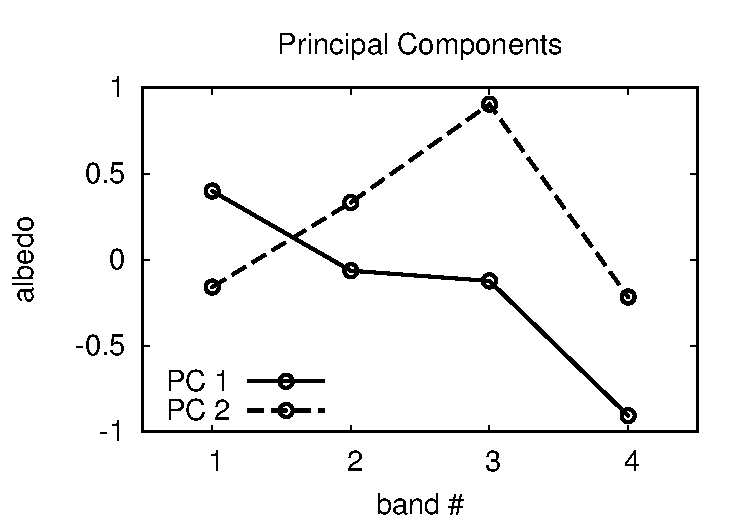
\includegraphics[width=\hsize]{PCA_V_jn.pdf}
%    \end{center}
%    \caption{Principal components of the light curves shown in the bottom of Figure \ref{fig:mockdata}. }
%\label{fig:PCs}
%\end{figure}
%%%%%%%%%%%%%%%%%%%%%%%%%%%%%%%%%%%

%%%%%%%%%%%%%%%%%%%%%%%%%%%%%%%%%%%
\begin{figure}[t]
    \begin{center}
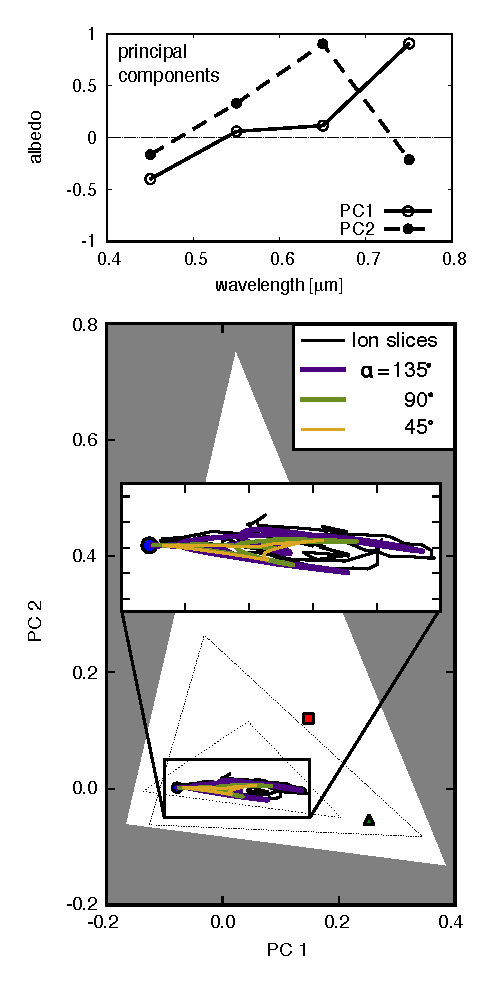
\includegraphics[width=\hsize]{mockdata_PCplane.pdf}
    \end{center}
    \caption{Upper panel: principal components (PCs) of the light curves at $\alpha = 90^{\circ }$ shown in olive lines in Figure \ref{fig:mockdata}. Lower panel: trajectories of the 4-band light curves on the PC plane set by 2 PCs shown in the upper panel, in the case of $\alpha = 135^{\circ }$ (indigo thick line), $\alpha = 90^{\circ }$ (olive line), and $\alpha = 45^{\circ }$ (gold thin line). Points indicate the input albedo spectra of ocean (blue circle), soil (red square), and vegetation (green triangle) on the PC plane. Points in the gray region violate the condition (\ref{eq:tilde_s_range}); specifically, the left, right, and bottom boundaries are set by $s_{k,4} > 0$, $s_{k,1} > 0$, and $s_{k,3}> 0$, respectively. 
Dotted lines are random triangle that could be solutions (see text). }
    \label{fig:trajectory}
\end{figure}
%%%%%%%%%%%%%%%%%%%%%%%%%%%%%%%%%%%

%%%%%%%%%%%%%%%%%%%%%%%%%%%%%%%%%%%%%%%%%%%%%%%%%%%%%%%%%%%%%%
\subsection{Formal Degeneracy}
\label{ss:degeneracy}
%%%%%%%%%%%%%%%%%%%%%%%%%%%%%%%%%%%%%%%%%%%%%%%%%%%%%%%%%%%%%%

On the other hand, when it comes to the stage where we must estimate the surface spectra given the trajectory/-ies, {\it any} set of $\{ {\bf s}_k \}$ that enclose the data points $\{{\bf d}_i\}$ in the hyperplane can be a solution of Equation (\ref{eq:tilde_d_f_ast_s}) subject to the conditions (\ref{eq:tilde_f_range}) and (\ref{eq:tilde_f_sum}). 
Note that the associated matrix, $\fast _{ik}$, can always be found. 

Additional constraints come from the condition (\ref{eq:tilde_s_range}). 
In Figure \ref{fig:trajectory} any points in the shadowed region are rejected based on this condition: specifically, the left, right, and bottom boundaries are set by $s_{k,4}> 0$, $s_{k,1}> 0$, and $s_{k,3}> 0$. 
While in this particular example the permitted region happens to be a triangle, shape can differ depending on the relative configuration of the boundaries\memoYF{In more detail?}. 
Although this limits the region where $\{ {\bf s}_k \}$ can exist,   
this is in general not sufficient to result in a unique solution. 

In Figure \ref{fig:trajectory} we show two random triangles that enclose the trajectory; these triangles satisfy the conditions (\ref{eq:tilde_f_range}) and (\ref{eq:tilde_f_sum}), as do many others. 
One can have spectrally interesting surface spectra and boring geography (small longitudinal variation in area fractions) {\it or} one can have boring surface spectra (closer to flat) and interesting geography. \memoYF{Need to reconsider this phrasing. }
Therefore, predicting ${\bf \fast }$ and ${\bf s}$ from ${\bf d}$ is clearly a ill-posed problem. 

A formally equivalent degeneracy is found in Equation (\ref{eq:d_f_s}) coupled with the conditions (\ref{eq:f_range})-(\ref{eq:s_range}). 
Essentially, the term $\sum _k f_{lk} s_{kj}$ represents the average albedo spectra of $l$-th slice and $W_{il}$ is the matrix that convolve them into the light curves. 
Suppose idealistically that we can retrieve the average spectra of longitudinal slices from the light curves through $W_{il}$; the trajectory in the panel C of Figure \ref{fig:trajectory} represents the color variation along the longitude.  
Again, we can have different sets of $\{ {\bf s}_k \}$ that enclose the averaged albedo spectra of longitudinal slices {\it and} are located in the range of condition (\ref{eq:s_range}), any of which can make up the given averaged albedo spectra with the associated $f_{lk}$. 
Nevertheless, the excursions of the longitudinal colors are more dramatic than the disk-integrated colors of the light curves, thus the possible solutions are somewhat more restricted. 
% For disk-integrated light curves, the color excursions are more muted than the intrinsic longitudinal map, so the degeneracy becomes severer. 


%%%%%%%%%%%%%%%%%%%%%%%%%%%%%%%%%%%%%%%%%%%%%%%%%%%%%%%%%%%%%%
\subsection{``Best Guess'' of the Surface Types}
\label{ss:guess}
%%%%%%%%%%%%%%%%%%%%%%%%%%%%%%%%%%%%%%%%%%%%%%%%%%%%%%%%%%%%%%


%%%%%%%%%%%%%%%%%%%%%%%%%%%%%%%%%%%
\begin{figure*}[tbh!]
   \begin{minipage}{0.33\hsize}
    \begin{center}
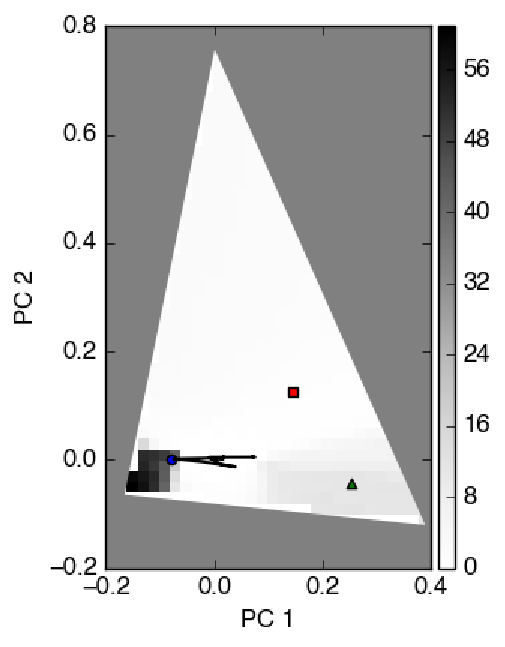
\includegraphics[width=\hsize]{mockdata_90deg_3types_t12_lc_noreg.pdf}
    \end{center}
     \end{minipage}   
    \begin{minipage}{0.33\hsize}
    \begin{center}
%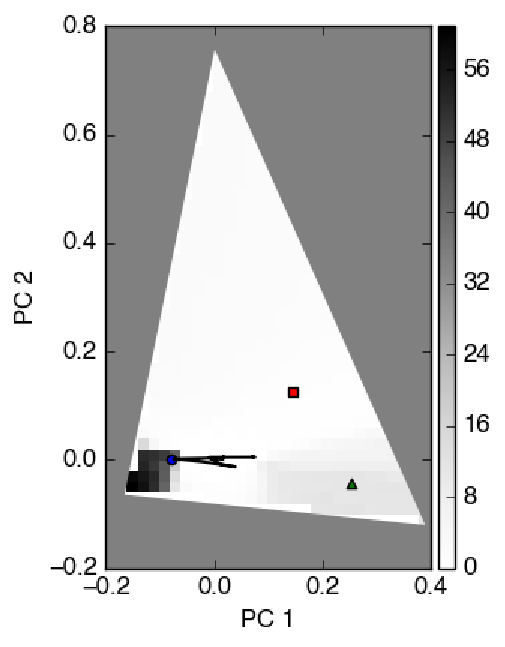
\includegraphics[width=\hsize]{mockdata_90deg_3types_t12_lc_noreg.pdf}
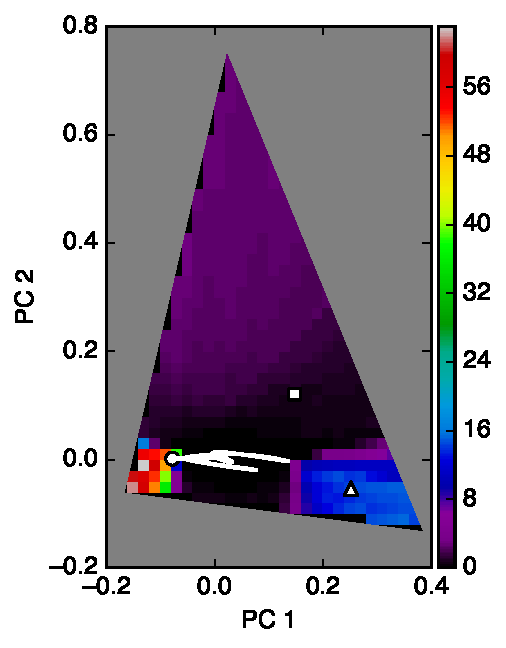
\includegraphics[width=\hsize]{mockdata_135deg_3types_t360_lc_noreg.pdf}
    \end{center}
     \end{minipage}
   \begin{minipage}{0.33\hsize}
    \begin{center}
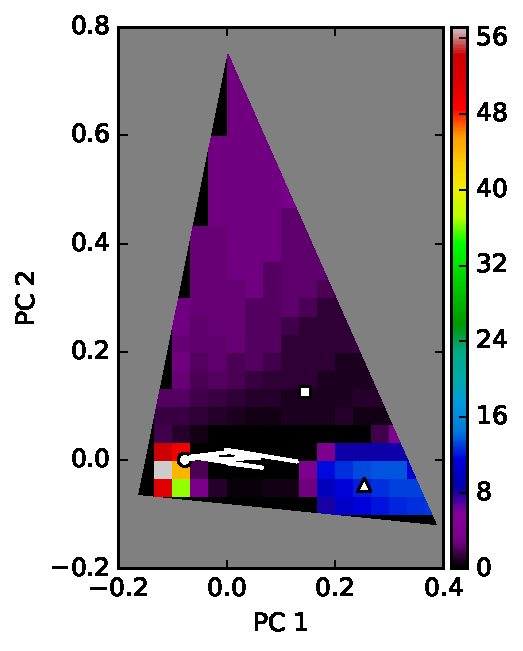
\includegraphics[width=\hsize]{IGBP_lon_noreg.pdf}
    \end{center}
     \end{minipage} 
   \begin{minipage}{0.33\hsize}
    \begin{center}
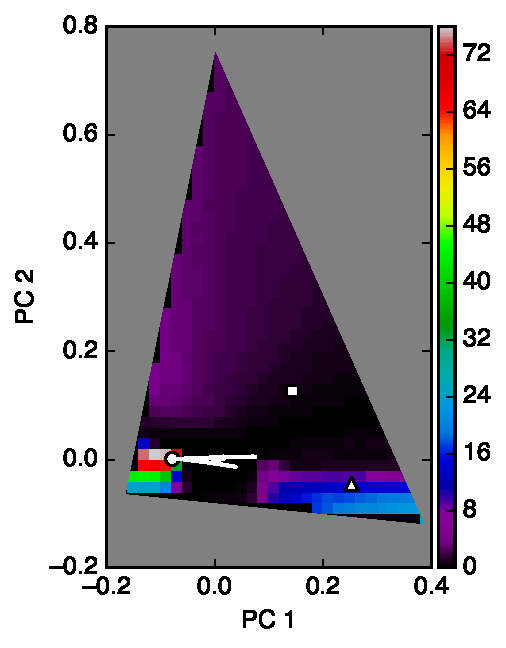
\includegraphics[width=\hsize]{mockdata_90deg_3types_t12_lc_reg_l30deg.pdf}
    \end{center}
     \end{minipage}      
   \begin{minipage}{0.33\hsize}
    \begin{center}
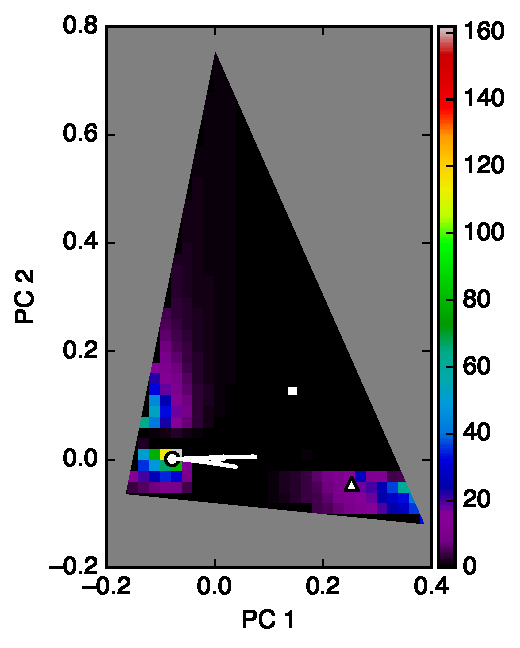
\includegraphics[width=\hsize]{mockdata_90deg_3types_t12_lc_reg_l40deg.pdf}
    \end{center}
     \end{minipage}
    \caption{(From top-left) A: Probability of surface albedo spectra estimated from the light curves of $\alpha = 90^{\circ }$ in the procedure described in Section \ref{ss:guess}. B: same as A but from the light curves of  $\alpha = 135^{\circ }$. C: same as A but from the colors of longitudinal slices.  D: same as A but from the light curves where the geographical maps of soil and vegetation are swaped. E: same as A but with regularization with $\Delta_ t = 2$ hr. F: same as A but with regularization with $\Delta_ t = 2.7$ hr. \memoYF{This is a tentative set of panels.} }
\label{fig:noreg}
\end{figure*}
%%%%%%%%%%%%%%%%%%%%%%%%%%%%%%%%%%%


Given that any vertices in the PC plane that enclose the trajectory/-ies can be a solution, the choice of the solution critically depends on the prior probability distribution. 
% Thus, we need to be careful about the implicit assumptions that are made  
With no assumptions or information on the spectral albedo of the surface types or geography, it may be reasonable to assume that any points in the PC plane except for the inhibited regions are equally likely to correspond to a surface type. 
%While such an assumption does not seem to work at all to choose the surface types, it does put some constrains. 
While such an assumption does not uniquely specify the colors of all $K$ surface types, it does offer constraints due to the relative light curve trajectory within the permitted region. 
%This is because of the relative configuration of the trajectory and the permitted region. 
For example, in Figure \ref{fig:trajectory}, in order to enclose the trajectory with three surface types within the permitted region, we must have at least one point near the bottom left corner of the permitted region (white triangle); this is consistent with the fact that one of the input albedo spectra (ocean) resides there. \memoJLY{and is a dominant surface type...?}


In order to see this more quantitatively, we make a grid on the PC plane  with an interval of 0.2 and consider all combinations of three grid points. 
Then, we assumed that all of the combinations that enclose the trajectory are equally likely to be a solution, and found the marginalized probability of having a surface type at each location of the PC plane. 
Specifically, we consider the following Bayesean expression and attempt to find the posterior distribution:
%%%
\begin{equation}
P_{\rm posterior} ( t_{kn} | U_{in} ) = P ( U_{in} | t_{kn} ) \cdot P_{\rm prior} (  t_{kn} ) 
\end{equation}
%%%
where $t_{kn}$ represents the coordinates of the $k$-th surface type on the PC plane ($n$ is either 1 or 2, corresponding to PC 1 and PC 2), i.e., 
%%%
\begin{equation}
s_{kj} = \sum_n t_{kn} V_{nj} + \bar d_j . 
\end{equation}
Assuming that any facet has the same prior probability per area of being a surface type, the prior for each $k$ is:
%%%
\begin{eqnarray}
&& P_{\rm prior} (t_{k1}, t_{k2} ) \, dt_{k1} dt_{k2} \\
&& = \left\{
\begin{array}{ll}
\displaystyle \frac{dt_{k1}  dt_{k2}}{\iint _{\rm allowed} d^2{\bf t}_k} & \;\;\;\;\;\; \mbox{if satisfies (\ref{eq:tilde_s_range})} \\
0 & \;\;\;\;\;\; \mbox{otherwise}
\end{array}
\right.
\end{eqnarray}
%%%
On the other hand, the likelihood is 
%%%
\begin{eqnarray}
&& P ( U_{in} | t_{kn} ) \\
&& \propto \left\{
\begin{array}{ll}
1 \;\;\; & \;\;\;\;\;\; \mbox{if satisfies (\ref{eq:tilde_f_range}) and (\ref{eq:tilde_f_range})} \\
0 \;\;\; & \;\;\;\;\;\; \mbox{otherwise}
\end{array}
\right.
\end{eqnarray}
%%%
Although the graphical meaning of conditions (\ref{eq:tilde_f_range}) and (\ref{eq:tilde_f_sum}) is simply to enclose the data, the judgement is numerically made as follows. 
We first find $\fast $ that satisfies condition (\ref{eq:tilde_f_sum}) from
%%%
\begin{equation}
\begin{pmatrix}
U_{11} & U_{12} & 1 \\
... & & 1 \\
U_{I1} & U_{I2} & 1 
\end{pmatrix}
= 
\begin{pmatrix}
\fast_{11} & \fast_{12} & \fast_{13}  \\
... & \\
\fast_{I1} & \fast_{I2} & \fast_{I3}
\end{pmatrix}
\begin{pmatrix}
t_{11} & t_{12} & 1 \\
t_{21} & t_{22} & 1 \\
t_{31} & t_{32} & 1 
\end{pmatrix}
\end{equation}
%%%
or,
\begin{equation}
\begin{pmatrix}
\fast_{11} & \fast_{12} & \fast_{13}  \\
... & \\
\fast_{I1} & \fast_{I2} & \fast_{I3}
\end{pmatrix}
=
\begin{pmatrix}
U_{11} & U_{12} & 1 \\
... & & 1 \\
U_{I1} & U_{I2} & 1 
\end{pmatrix}
\begin{pmatrix}
t_{11} & t_{12} & 1 \\
t_{21} & t_{22} & 1 \\
t_{31} & t_{32} & 1 
\end{pmatrix}^{-1}
\label{eq:f=ds-1}
\end{equation}
%%%
Note that the last matrix is a $K\times K$ matrix, and thus inverse is found if $\{ {\bf t}_k \}$ forms a triangle (rather than a straight line or a single dot, in which case $\{ {\bf t}_k \}$ is not a solution anyways).
Then, we ask if the resultant $\fast_{ik}$ are within the range of (\ref{eq:tilde_f_range}). 

Finally, we marginalize the posterior distribution, i.e.,
%%%
\begin{equation} 
P_{\rm posterior} ( {\bf t}_1) = \iint P_{\rm posterior} ( t_{kn} | d_{ij} ) d^2 {\bf t}_2 d^2 {\bf t}_3
\end{equation}
%%%
given the symmetry of ${\bf t}_1$, ${\bf t}_2$, and ${\bf t}_3$. 
$P_{\rm posterior} ( {\bf t}_1) $ is normalized so that it sums up to unity. 

The resultant probability distribution is shown in Figure \ref{fig:noreg}. 
As expected, we find a relatively definite peak near the point of ocean. 
On the other hand, the peak that corresponds to soil is a blur, and it is almost not constrained. 
The vegetation in the bottom right corner is moderately constrained. 

We iterate that in this framework the success of the guess critically depends on the relative configuration of the trajectory and allowed region. 
In panel D of Figure \ref{fig:noreg}, we show another example where we switched the geographical map of soil and vegetation; as a result, the trajectory moves toward soil rather than vegetation. However, because the allowed region near the soil is large, soil is still not sufficiently constrained. 


%%%%%%%%%%%%%%%%%%%%%%%%%%%%%%%%%%%%%%%%%%%%%%%%%%%%%%%%%%%%%%
\subsection{Additional Assumptions}
\label{ss:regularization}
%%%%%%%%%%%%%%%%%%%%%%%%%%%%%%%%%%%%%%%%%%%%%%%%%%%%%%%%%%%%%%

\memoYF{I still have some concerns about this and the text needs revision. }

A possible constraining assumption we might make is the correlation length of the area fraction as a function of time, or as a function of longitude.  
Smooth time or longitudinal variation with correlation lengths may be imposed as Gaussian Process \citep{Rasmussen2005}, which means the any finite number of the covering fractions have a joint Gaussian distribution. 
In our case, the prior for $f_{lk}$ for each $k$ is then:
%%%
\begin{eqnarray}
&& P_{\rm prior} (  \fast_{1k}, \fast_{2k}, ..., \fast_{Ik} ) \\
&& \propto \frac{1}{\sqrt{| \tilde \Sigma^{(k)} |}}  \exp\left[ - (\fast^{T})_{ki} ( \tilde \Sigma ^{(k)} )^{-1}_{ii'} \fast_{i'k} \right]
\end{eqnarray}
%%%
where
%%%
\begin{equation}
\tilde \Sigma _{ll'} = \lambda \exp \left( - \frac{|t_i- t_i'|^2}{2 \Delta_ t^2} \right)
\end{equation}
%%%
or
%%%
\begin{eqnarray}
&& P_{\rm prior} (  f_{1k}, f_{2k}, ..., f_{Lk} ) \\
&& \propto \frac{1}{\sqrt{| \Sigma^{(k)} |}}  \exp\left[ - (f^{T})_{kl} ( \Sigma ^{(k)} )^{-1}_{ll'} f_{l'k} \right]
\end{eqnarray}
%%%
where
%%%
\begin{equation}
\Sigma _{ll'} = \lambda \exp \left( - \frac{|\phi_l- \phi_{l'}|^2}{2 \Delta _{\phi }^2} \right). 
\end{equation}
%%%

The posterior will be
%%%
\begin{eqnarray}
P_{\rm posterior} ( t_{kn} | d_{ij} ) &=& P ( d_{ij} | t_{kn}, f_{lk} ) \\
&& \times \, P_{\rm prior} (  t_{kn} ) P_{\rm prior} (  f_{lk} ) \\
P ( d_{ij} | t_{kn}, f_{lk} ) &=& \delta( f_{lk} - f_{lk}^{(0)} (t_{kn}) )
\end{eqnarray}
%%%
where $f_{lk}^{(0)}$ is the solution of Equation (\ref{eq:f=ds-1}). 
\memoYF{Very acrobatic. Am I doing right? I am not sure.}

Panel E and F of Figure \ref{fig:noreg} are the results where $\Delta_ t = 2$ hr and $2.7$ hr, respectively. 
In this case, we find the higher peak of albedo spectra of ocean closer to the ``answer'', while the vegetation is identified far off the ``answer''; vegetation is intermediate. 

We must take caution here that the actual covering fraction of surface types do not necessarily obey gaussian process. 
In this particular case, it appears that the dominant surface type (ocean) is better approximated by gaussian processes.... \memoYF{??}


\memoYF{Have to do with regularization on the maps, but how should we proceed without doing MCMC with both $f_{lk}$ and $s_{kj}$ being fitting parameters? I could operate $W^{+}_{li} \fast_{ik}$ to find $f_{lk}$ with condition (\ref{eq:f_range}) and (\ref{eq:f_sum}); this itself is a bounded linear inversion problem and thus needs some minimization. Also, without regularization, I tend to find scattered $f_{lk}$, perhaps because of the instability of inverse matrix??. }


%%%%%%%%%%%%%%%%%%%%%%%%%%%%%%%%%%%%%%%%%%%%%%%%%%%%%%%%%%%%%%
\section{Application to EPOXI data}
\label{s:EPOXI}
%%%%%%%%%%%%%%%%%%%%%%%%%%%%%%%%%%%%%%%%%%%%%%%%%%%%%%%%%%%%%%

%%%%%%%%%%%%%%%%%%%%%%%%%%%%%%%%%%%
\begin{figure}[tbh!]
    \begin{center}
	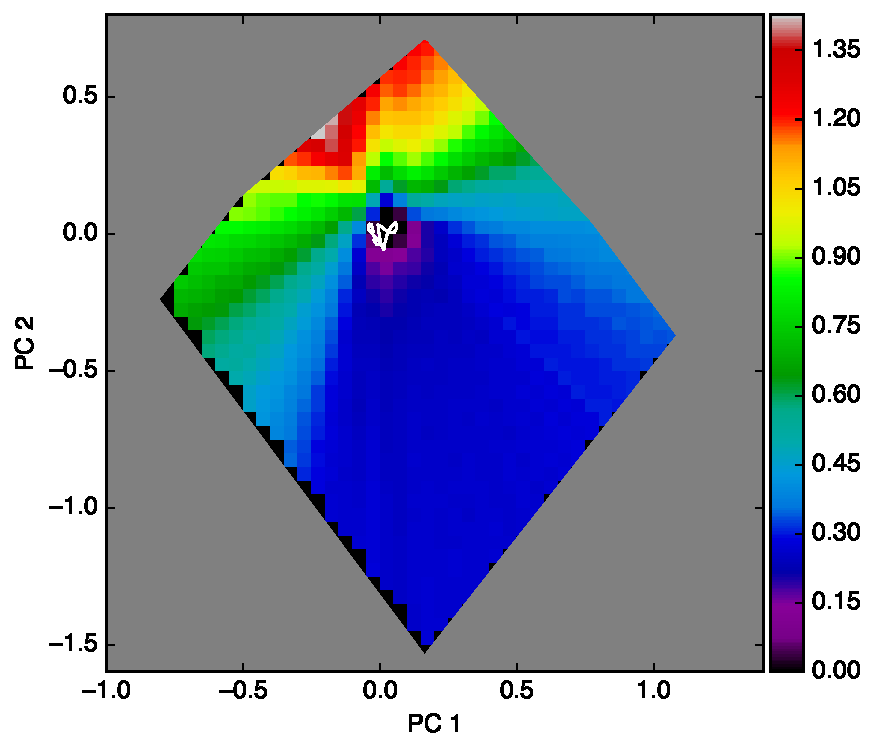
\includegraphics[width=\hsize]{raddata_2_PCplane_noreg.pdf}
    \end{center}
    \caption{PC plane from EPOXI observation of June 2008. }
\label{fig:EPOXI}
\end{figure}
%%%%%%%%%%%%%%%%%%%%%%%%%%%%%%%%%%%



In this section, we apply our analysis procedure to the observed multi-band light curves of the Earth observed by EPOXI mission. 
Specifically we use the same datasets as \citet{Cowan2013}, i.e., the 7-band diurnal light curves observed in June of 2008 \citep{Livengood2011}. 
Using two dominant PCs we extracted, we performed the same analysis described in the previous section 

Figure \ref{fig:EPOXI} shows the trajectory of the light curve projected onto the PC plane, with the grayed region being the forbidden region. 
While the permitted region appears to be close to a square, it is in fact a heptagon, bounded by 7 inequalities. Overall, the upper boundaries come from the requirement of $s_{kj}>0$ while the lower boundaries comes from the requirement of $s_{kj}<1$. 

In this case, the trajectory of planetary light curves is away from the boundary because the color variations of the real Earth are muted by the cloud cover \memoYF{True?}. 
Consequently, we do not see three peaks but a spectrum of the potential. 
Nevertheless, we are likely to find one surface type near the upper right part of the allowed region. 

%%%%%%%%%%%%%%%%%%%%%%%%%%%%%%%%%%%
\begin{figure}[tbh!]
    \begin{center}
	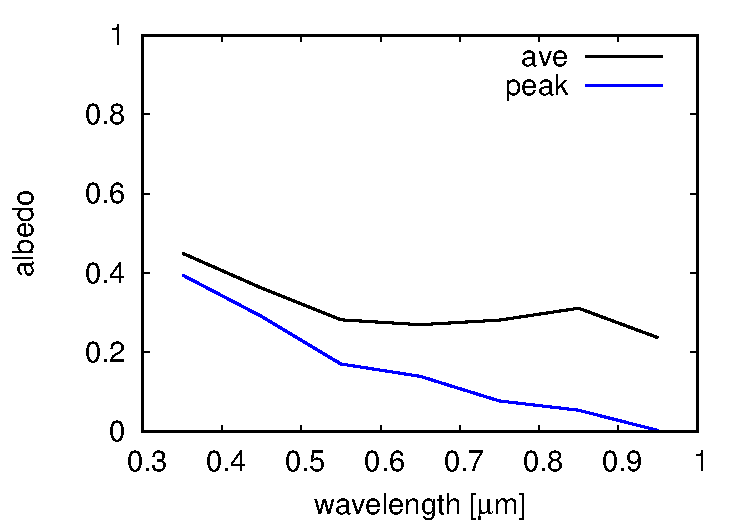
\includegraphics[width=\hsize]{raddata_2_norm_Mj_PCs.pdf}
    \end{center}
    \caption{Albedo spectra of the upper left peak in Figure \ref{fig:EPOXI}. }
\label{fig:EPOXI}
\end{figure}
%%%%%%%%%%%%%%%%%%%%%%%%%%%%%%%%%%%





%%%%%%%%%%%%%%%%%%%%%%%%%%%%%%%%%%%%%%%%%%%%%%%%%%%%%%%%%%%%%%
\section{Discussion}
\label{s:discussion}
%%%%%%%%%%%%%%%%%%%%%%%%%%%%%%%%%%%%%%%%%%%%%%%%%%%%%%%%%%%%%%

\memoYF{This section could be merged with Conclusion section.}

\subsection{Effect of Uncertain Planetary Radius and Orbit}

So far we have assumed that the geometrical parameters are completely known, including the planetary orbit, planetary spin axis and the planetary radius. 
% In this section we discuss the influence of incomplete knowledge of these parameters. 
How would the uncertainties in these parameters affect our retrieval?
In fact, the decomposition into $\fast $ and $s$ does not require the information of spin axis or spin period. 
What matters most in this case is the uncertainty in the normalization of apparent albedo. 
In reality, direct imaging observations alone provide the intensity of the 
planetary light and the intensity of the stellar light, and in order to convert this to the unit of albedo we need to know the orbital distance from the star, phase angle, and planetary radius. 
If there are uncertainties in these estimates, the relative configuration among the light curve trajectories, the boundaries coming from $s_{jk} < 1$, and those coming from $s_{jk} > 0$ are changed, thus the estimates can be substantially biased. 

\subsection{Deviation from Lambert's Law}

We have assumed that the scattering by surface obeys Lambert's law, but in reality they are not perfect Lambert scatterers, as noted. 
In particular, scattering by ocean exhibits prominent specular reflection and the reflectivity increases when the incident light is grazing, or equivalently at crescent phase \citep[e.g.,][]{Williams2008}. 
Furthermore, when we take account of an atmosphere above the surface, the albedo spectra of surface overlaid by an atmosphere changes in phase angle.  
Considering these effects, the trajectories of the light curves at different phases do not have to reside in the same PC plane. 
These light curves can be analyzed independently, and the components varying with phase would rather give us insights into the anisotropic scatterers. 

%\memoYF{Problem in inverse matrix...!}

%%%%%%%%%%%%%%%%%%%%%%%%%%%%%%%%%%%%%%%%%%%%%%%%%%%%%%%%%%%%%%
\section{Conclusion}
\label{s:conclusion}
%%%%%%%%%%%%%%%%%%%%%%%%%%%%%%%%%%%%%%%%%%%%%%%%%%%%%%%%%%%%%%

In this paper, we revisited the framework to estimate the albedo spectra of major surface types of exoplanets and their distribution from disk-integrated multi-band photometric data. 
We pointed out the inherit degeneracy which makes it impossible to find unique solutions. 
While admitting the degeneracy, some constraints about the likely solutions may be found, owing to the nature of albedo which is between 0 and 1. 
We demonstrate using a simplified toy model of the Earth that such constraints work in some cases. 
...
%The constraints can be...



\bibliography{ref}

\appendix


%%%%%%%%%%%%%%%%%%%%%%%%%%%%%%%%%%%%%%%%%%%%%%%%%%%%%%%%%%%%%%
\section{Swapping Geographical Maps}
%%%%%%%%%%%%%%%%%%%%%%%%%%%%%%%%%%%%%%%%%%%%%%%%%%%%%%%%%%%%%%

% In this section we demonstrate how the albedo spectra and geographical maps of the surface types affect our retrieval. 
In our fiducial model, i.e., Figure \ref{fig:noreg}, the color of ocean was best constrained. 
%
This appears to be due to the combination of the large covering fraction of ocean and the location of the color of ocean in the PC plane. 
To illustrate these two effects, we created two additional mock light curves, (a) with the geographical maps of the soil and vegetation being swapped, and  (b) with the geographical maps of the soil and ocean being swapped. 
The left and right panels of Figure \ref{fig:swap} correspond to (a) and (b), respectively. 
%
When we swap soil and vegetation, i.e., (a), the covering fraction of vegetation becomes smaller, and the trajectory of the light curves come toward the color of vegetation only a little bit. As a result, the constraints of the color of vegetation becomes weaker. Thus, a large covering fraction of the surface type tend to yield a better constraint on the albedo spectra of that type. 
%
In the meanwhile, in (b) where we swapped the soil and ocean, although soil is the dominant component, the true location of the soil is rather not preferred based on our analysis to other locations toward the top, because there are larger space there. 
Therefore, large covering fraction is not a sufficient condition to better constrain the spectral albedo. 

%%%%%%%%%%%%%%%%%%%%%%%%%%%%%%%%%%%
\begin{figure}[tbh!]
    \begin{center}
   \begin{minipage}{0.33\hsize}
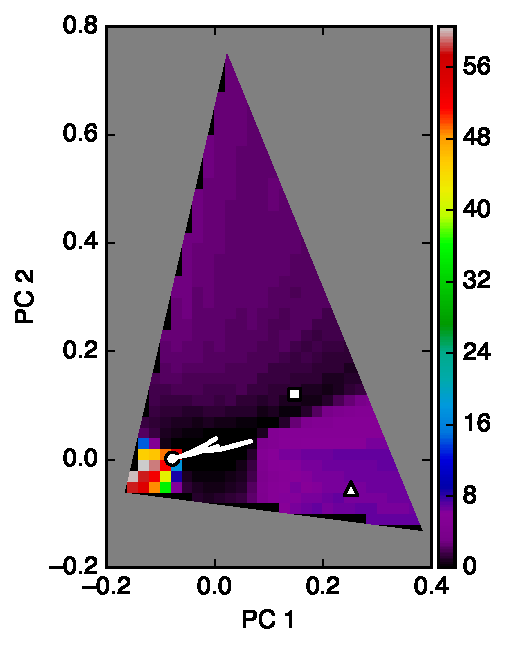
\includegraphics[width=\hsize]{mockdata_90deg_3types2_t360_lc_noreg.pdf}
     \end{minipage}
   \begin{minipage}{0.33\hsize}
%    \begin{center}
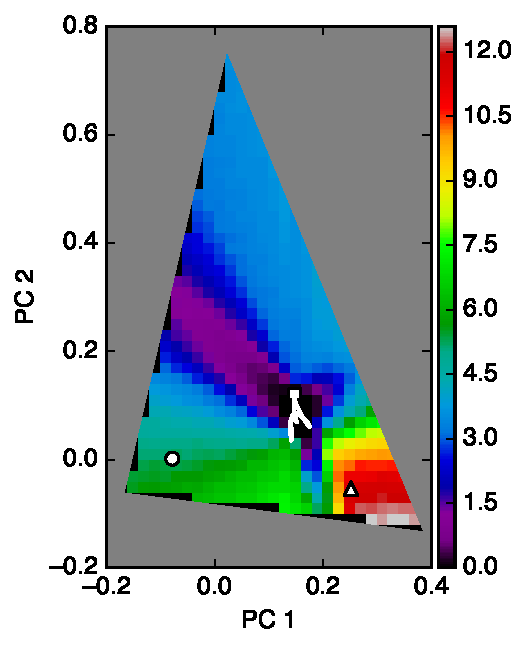
\includegraphics[width=\hsize]{mockdata_90deg_3types3_t360_lc_noreg.pdf}
%    \end{center}
     \end{minipage}
    \end{center}
    \caption{Left: Trajectory of the light curves with the geographical maps of the soil and vegetation being swapped, and the resultant color contour of the posterior probability of albedo spectra of surface types. (b) Same as (a) but with the geographical maps of the soil and ocean being swapped. }
\label{fig:swap}
\end{figure}
%%%%%%%%%%%%%%%%%%%%%%%%%%%%%%%%%%%


%%%%%%%%%%%%%%%%%%%%%%%%%%%%%%%%%%%%%%%%%%%%%%%%%%%%%%%%%%%%%%
\section{Difficulty in Longitudinal Observations}
%%%%%%%%%%%%%%%%%%%%%%%%%%%%%%%%%%%%%%%%%%%%%%%%%%%%%%%%%%%%%%

\memoYF{Looking for better description. }

The difficulty in color retrieval from the rotational light curves is simply that we cannot resolve the planetary surface with high spatial resolution; if we had extremely high spatial resolution of the planetary surface, the colors of individual surface patches would be well represented by the colors of either ocean, soil, or vegetation, and it is trivial to identify the surface types. 
Figure \ref{fig:lowresolution} displays how the lowering the spatial resolution of the map mixes the colors of individual pixels, using HEALPix pixelization. 
From left to right, we change the resolution from 192 pixels, 48 pixels to 12 pixels, based on the top panel of Figure \ref{fig:mockdata}. 
As expected, the fraction of pixels with intermediate colors increases as we lower the resolution. 
When the number of pixel is as small as 12, there is no longer a pixel composed purely of soil or vegetation. 
With 48 pixels, the triangle shape is marginally seen. 

In the case of observations of diurnal light curves, as we go closer to crescent phase, the illuminated and visible area becomes narrower and the colors go more extreme (Figure \ref{fig:trajectory}), which is better  constraining the colors of the surface types. 
However, changing the width of the illuminated and visible are is different from changing the spatial resolution using HEALPix as described above. 
This is because even at crescent phase, colors of very distant pixels, beyond the correlation length of the geography, are mixed together---for example, the color of the North Pole and that of South Pole are merged in an equatorial observation, no matter how thinner phase we observe. 
% On the other hand, lowering resolution in HEALPix maintain the 
Figure \ref{fig:lowresolution} should thus be compared with the trajectory in the upper right panel of Figure \ref{fig:noreg}, which is the colors of 360 longitudinal slices (width: $1^{\circ }$). 
Despite the number of slices, the colors of individual slices minimally get close to the location of vegetation or soil. 
This limits our ability to retrieve the surface types. 


%%%%%%%%%%%%%%%%%%%%%%%%%%%%%%%%%%%
\begin{figure*}[tbh!]
   \begin{minipage}{0.33\hsize}
    \begin{center}
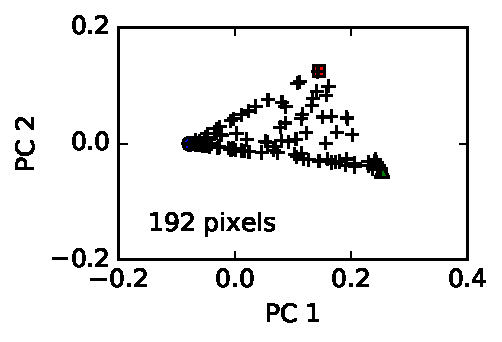
\includegraphics[width=\hsize]{IGBP_PCplane_Nside2.pdf}
    \end{center}
     \end{minipage}   
    \begin{minipage}{0.33\hsize}
    \begin{center}
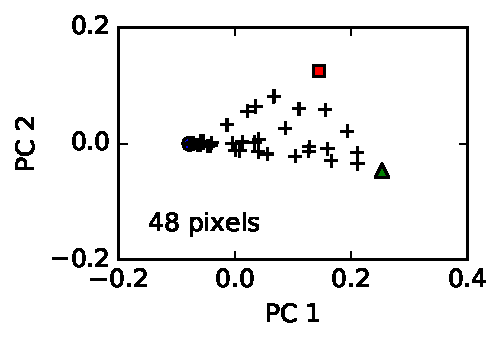
\includegraphics[width=\hsize]{IGBP_PCplane_Nside1.pdf}
    \end{center}
     \end{minipage}
   \begin{minipage}{0.33\hsize}
    \begin{center}
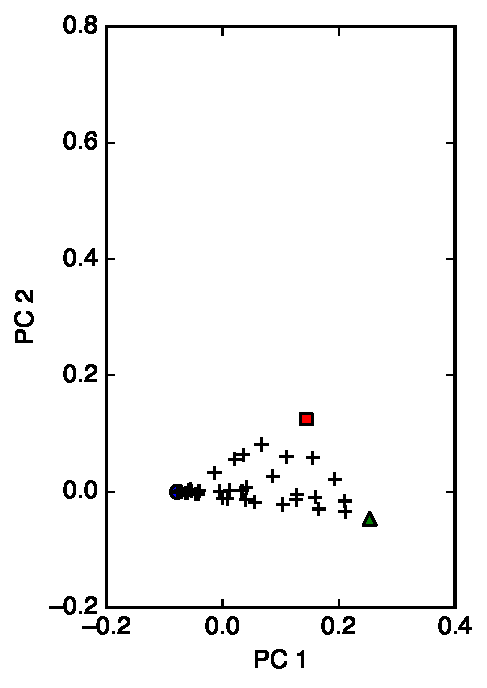
\includegraphics[width=\hsize]{IGBP_PCplane_Nside0.pdf}
    \end{center}
     \end{minipage}
    \caption{Making the map coarser using HealPix. Left: 192 pixels, Middle: 48 pixels, Right: 12 pixels. }
\label{fig:lowresolution}
\end{figure*}
%%%%%%%%%%%%%%%%%%%%%%%%%%%%%%%%%%%



\end{document}
